% Use the following line  only  if you're still using LaTeX 2.09.
%\documentstyle[icml2014,epsf,natbib]{article}
% If you rely on Latex2e packages, like most moden people use this:
\documentclass{article}
% use Times
\usepackage{times}
 % For figures
\usepackage{graphicx} % more modern
%\usepackage{epsfig} % less modern
\usepackage{subfigure} 
\usepackage{footnote}
\usepackage{amsfonts}
\usepackage{mdframed}

% For citations
\usepackage{natbib}
\usepackage{comment}
\usepackage{multirow}

\usepackage{float}

\floatstyle{plain} % optionally change the style of the new float
\newfloat{code}{H}{myc}

% For algorithms
\usepackage{algorithm}
\usepackage{algorithmic}
\usepackage{amsmath}
\usepackage{listings}

\lstset{language=Python,
  basicstyle=\ttfamily\footnotesize,
  keywordstyle=\color{blue}\ttfamily,
  stringstyle=\color{red}\ttfamily,
  commentstyle=\color{green}\ttfamily,
  aboveskip=0pt,
  belowskip=0pt,
  breaklines=true
}

\setlength{\abovedisplayskip}{0cm}
\setlength{\belowdisplayskip}{0cm}

\usepackage{mathtools}


\newcommand\myeq{\stackrel{\mathclap{\normalfont\mbox{{\tiny def}}}}{=}}


\usepackage[compact]{titlesec}
\titlespacing{\section}{0pt}{0.5ex}{0.3ex}
\titlespacing{\subsection}{0pt}{0.2ex}{0ex}
\titlespacing{\subsubsection}{0pt}{0.1ex}{0ex}

\newcommand{\startcompact}[1]{\par\vspace{-0.75em}\begin{#1}%
  \allowdisplaybreaks\ignorespaces}

\newcommand{\stopcompact}[1]{\end{#1}\ignorespaces}

\usepackage{paralist}

\makeatletter
\ifcase \@ptsize \relax% 10pt
  \newcommand{\miniscule}{\@setfontsize\miniscule{4}{5}}% \tiny: 5/6
\or% 11pt
  \newcommand{\miniscule}{\@setfontsize\miniscule{5}{6}}% \tiny: 6/7
\or% 12pt
  \newcommand{\miniscule}{\@setfontsize\miniscule{5}{6}}% \tiny: 6/7
\fi
\makeatother

\newcommand {\aplt} {\ {\raise-.5ex\hbox{$\buildrel<\over\sim$}}\ }

\newcommand{\eqn}[1]{Eqn.~\ref{eqn:#1}}
\newcommand{\fig}[1]{Fig.~\ref{fig:#1}}
\newcommand{\tab}[1]{Table~\ref{tab:#1}}
\newcommand{\secc}[1]{Section~\ref{sec:#1}}
\def\etal{{\textit{et~al.~}}}
\newcommand{\BigO}[1]{\ensuremath{\operatorname{O}\left(#1\right)}}
\usepackage[symbol*]{footmisc}

\DefineFNsymbolsTM{myfnsymbols}{% def. from footmisc.sty "bringhurst" symbols
  \textasteriskcentered *
  \textdagger    \dagger
  \textdaggerdbl \ddagger
  \textsection   \mathsection
  \textbardbl    \|%
  \textparagraph \mathparagraph
}%


% As of 2011, we use the hyperref package to produce hyperlinks in the
% resulting PDF.  If this breaks your system, please commend out the
% following usepackage line and replace \usepackage{icml2014} with
% \usepackage[nohyperref]{icml2014} above.
\usepackage{hyperref}

% Packages hyperref and algorithmic misbehave sometimes.  We can fix
% this with the following command.
\newcommand{\theHalgorithm}{\arabic{algorithm}}

% Employ the following version of the ``usepackage'' statement for
% submitting the draft version of the paper for review.  This will set
% the note in the first column to ``Under review.  Do not distribute.''
%\usepackage{icml2014} 
% Employ this version of the ``usepackage'' statement after the paper has
% been accepted, when creating the final version.  This will set the
% note in the first column to ``Proceedings of the...''
\usepackage[accepted]{icml2014}



\begin{document} 

\twocolumn[
\icmltitle{Learning to Reason\\{\small PhD Thesis Proposal}}

\icmlauthor{Wojciech Zaremba}{woj.zaremba@gmail.com}
\vskip +0.1in
\icmlauthor{Advisors:}{}
\vskip +0.03in
\icmlauthor{Rob Fergus}{fergus@cs.nyu.edu}
\vskip +0.03in
\icmlauthor{Yann LeCun}{yann@cs.nyu.edu}
\icmladdress{New York University}

\icmlkeywords{computer vision, convolutional neural networks, recurssive neural networks, natual language processing, recurrent neural networks, language model, LSTMs, program understanding, artificial intelligence}

\vskip 0.3in
]

\begin{abstract}

Neural networks proven to be a very powerful models for object recognition \cite{krizhevsky2012imagenet}, 
natural language processing \cite{mikolov2012statistical}, speech recognition \cite{graves2013speech}, and many others \cite{sutskever2014sequence}. 
However, there is still a huge gap between them, and an intelligent systems. 
I identify several potential unaddressed skills, which intelligent systems should possess: 
(1) reasoning abilities, (2) capability to integrate with external interfaces and (3) small sample complexity. My research focuses on tackling this problems. 

\end{abstract} 

\section{Introduction}
It's clear that by improving performance of current statistical learning systems, 
we won't be able to make them intelligent. Even if our object recognition system would yield
$0\%$ of prediction error, they wouldn't be intelligent. Same applies to speech 
recognition systems, machine translation and others. This work asks what skills are necessary for statistical
learning system to become ``intelligent''. Moreover, it attempts to address this remaining unaddressed skills. 


I believe, that crucial, poorly addressed skills that intelligent system has to poses are
(1) reasoning abilities, (2) capability to integrate with external interfaces and (3) small sample complexity. 
I would like to address all this problems within seamless system. The same system should be used across
different tasks, and should be able to emulate simpler models. 


I have partially addressed some of proposed problems. I am referring to my work, and I am defining future goals.




\section{Reasoning abilities}

Reasoning - ``the process of forming conclusions, judgments, or inferences from facts or 
premises'' \footnote{Definition from \url{http://dictionary.reference.com/browse/reasoning}}.







There exists many rule based reasoning systems. 
However, intelligent system reasoning cannot be based only on predefined rules. 
It has to be based on pattern matching, and application of learnt heuristic algorithms. 
I would like to build a statistical reasoning system. 


There are many domains where it is crucial. Domains of my interest include learning object relations in computer vision, proving mathematical theorems, and learning about computer programs.

\subsection{Reasoning in computer programs}

\begin{figure}
  \begin{code}
  \begin{mdframed}
  {\bf Input:}
  \begin{lstlisting}
  f=(8794 if 8887<9713 else (3*8334))
  print((f+574))
  \end{lstlisting} 
  {\bf Target:} 9368. \\
  {\bf Model prediction:} 9368. 
  \end{mdframed}
  \end{code}
  \caption{aaa}
\end{figure}



\subsection{Reasoning in mathematics}

\begin{figure}
  \centering
  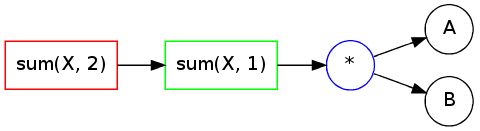
\includegraphics[width=0.48\textwidth]{imgs/example1_brute.png}\\
  {\bf Is equivalent to:}\\
  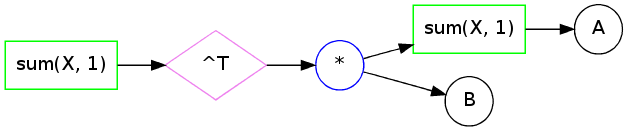
\includegraphics[width=0.48\textwidth]{imgs/example1_opt.png}\\
  \caption{\cite{zaremba2014learning}}
\end{figure}


\subsection{Reasoning in computer vision}

\begin{figure}
  \centering
  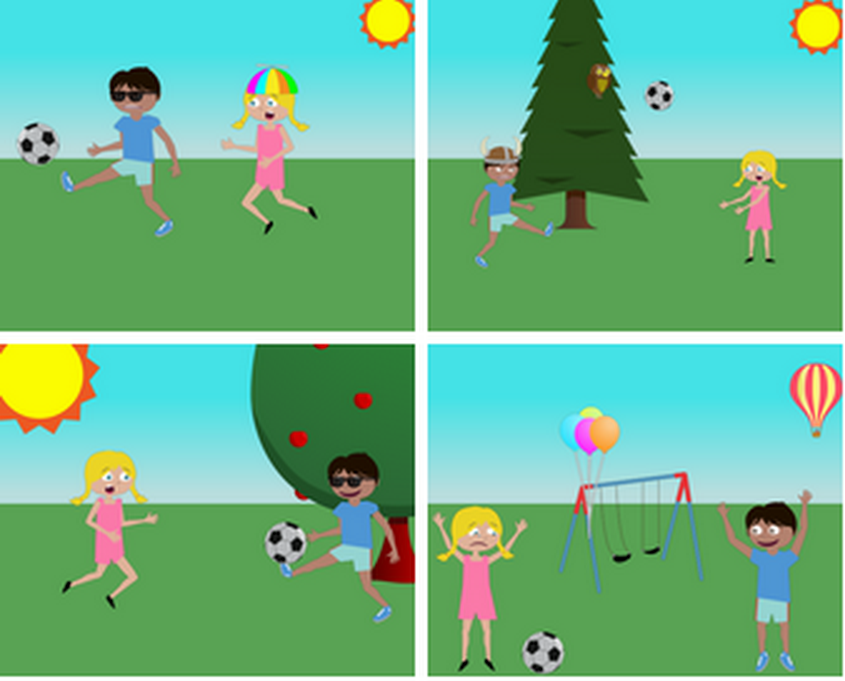
\includegraphics[width=0.48\textwidth]{imgs/abstract.png}\\
  \caption{Jenny loves to play soccer but she is worried that Mike will kick the ball too hard.}
\end{figure}

\section{Interface learning}
Contemporary machine learning systems are closed in a box, and cannot 
interact with external interfaces. 


Initial advances in machine learning, where lead by engineering features, 
e.g histogram of colors, SIFT (Scale-invariant feature transform) features. 
This approach has its limitations, and its fragile. Moreover, it requires a 
human expert to train the system for the every new domain. Ideal system should 
have access to external interfaces that might give access to information, or simplify it processing. 
Interfaces that I have in mind are following (1) grid that helps to process images, (2) search engine, 
(4) Linux syscalls, or (5) execution environment like python interpreter. External interfaces are not-differentiable, 
and their state space is massive. This obstacles could potentially be addressed by learning a differentiable 
model that describes them (e.g. neural network). Neural network would simulate such external interface in a model-based reinforcement learning approach. 

\section{Toward all tasks one-shot learning}
Current deep learning systems suffer of large sample complexity. Such 
high sample complexity hinders potential use of the systems in online 
learning systems (e.g. robots). It’s expected that during the initial phase of 
learning any system without prior knowledge would need to consume a large number of samples. 
We hope that over the time of training, sample complexity should drop. However, this is 
not observed in current systems. I would like to build a meta-optimizer that could 
overcome this limitation. Such optimizer would consume gradients of a neural network, 
and would decide on the next update step. Optimizer itself could be parameterized 
with a neural network. Proper weights could simulate any first order, gradient-based, 
learning algorithm like SGD, momentum, LBFGs etc. This implies that meta-optimizer 
subsumes all first order, gradient-based optimization techniques. Trained meta-optimizer 
could update the network in a much more clever way, and a single sample could provide enough knowledge.



\section{Discussion}
Tackling aforementioned problems would take us much closer to the
real intelligent systems, and defines for me the three main pillars 
of artificial intelligence. However, there are many other problems, which 
would need to be solved / integrated within such system to make it fully 
intelligent, e.g. navigation, learning by imitation, cooperation, and many others.


\bibliography{bibliography}
\bibliographystyle{icml2014}

\end{document} 

